\documentclass{ximera}
\usepackage{../OERLinearAlgebra}


\usepackage{mathtools}
\usepackage{tikz-3dplot}
\newcommand\norm[1]{\left\lVert#1\right\rVert}

\author{Anna Davis \and Rosemarie Emanuele} \title{A Brief Introduction to $\RR^n$} \license{CC-BY 4.0}

\begin{document}

\begin{abstract}
 We define $\RR^n$ and learn how to plot points in $\RR^3$.
\end{abstract}
\maketitle


The set of all real numbers is denoted by $\RR$.  It is convenient to associate real numbers with points on a line, called the {\it real number line}.   

\begin{image}
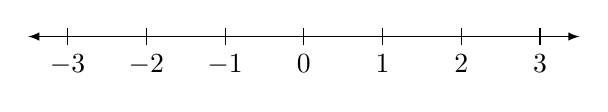
\begin{tikzpicture}
\draw[latex-latex] (-3.5,0) -- (3.5,0) ; %edit here for the axis
\foreach \x in  {-3,-2,-1,0,1,2,3} % edit here for the vertical lines
\draw[shift={(\x,0)},color=black] (0pt,3pt) -- (0pt,-3pt);
\foreach \x in {-3,-2,-1,0,1,2,3} % edit here for the numbers
\draw[shift={(\x,0)},color=black] (0pt,0pt) -- (0pt,-3pt) node[below] 
{$\x$};
\end{tikzpicture}
\end{image}

The set of all ordered pairs $(x, y)$, where $x$ and $y$ are real numbers is called $\RR^2$.  Using set notation we write:  
$$\RR^2=\{(x, y)|x,y\in \RR\}$$
Geometrically speaking, $\RR^2$ can be associated with a coordinate plane in which we refer to each point by its $x$ and $y$ coordinates.
\begin{image}
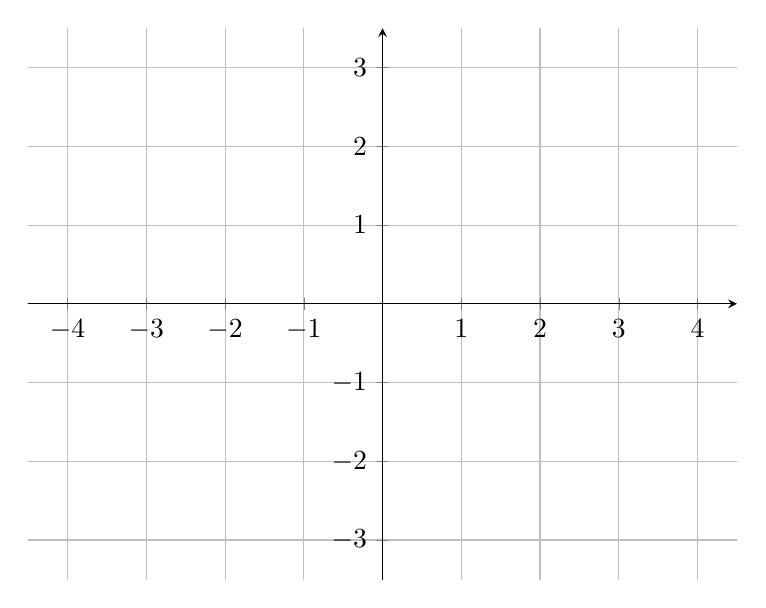
\begin{tikzpicture}[line cap=round,line join=round,>=triangle 45,x=1cm,y=1cm]
\begin{axis}[
x=1cm,y=1cm,
axis lines=middle,
ymajorgrids=true,
xmajorgrids=true,
xmin=-4.5,
xmax=4.5,
ymin=-3.5,
ymax=3.5,
xtick={-4,-3,...,4},
ytick={-3,-2,...,3},]
\end{axis}
\end{tikzpicture}
\end{image}
The set of all ordered triples $(x, y, z)$, where $x$, $y$ and $z$ are real numbers,  is called $\RR^3$.  
$$\RR^3=\{(x, y, z)|x,y, z\in \RR\}$$
Geometrically, points of $\RR^3$ are associated with points of a three-dimensional space whose position is given by their $x$, $y$ and $z$ coordinates.

\begin{image}[2in]
\tdplotsetmaincoords{70}{130}
\begin{tikzpicture}
	\draw[->](-2,0,0)--(5,0,0) node[below left]{$y$};
    \draw[->](0,-2,0)--(0,5,0) node[below left]{$z$};
    \draw[->](0,0,-2)--(0,0,5) node[below left]{$x$};
    
   \end{tikzpicture}
\end{image}

\begin{example} The following points are shown plotted in $\RR^3$.

  \begin{enumerate}
\item
$P(6, 8, 7)$
\item
$Q(4, -6, 9)$
\item
$R(-3, 9, -10)$
  \end{enumerate}
  
  
  \begin{image}[4.5in]
\begin{tikzpicture}[x=0.5cm,y=0.5cm,z=0.3cm]
% The axes
\draw[->] (xyz cs:x=-13.5) -- (xyz cs:x=13.5) node[above] {$y$};
\draw[->] (xyz cs:y=-13.5) -- (xyz cs:y=13.5) node[right] {$z$};
\draw[->] (xyz cs:z=13.5)--(xyz cs:z=-13.5) node[below] {$x$} ;
% The thin ticks
\foreach \coo in {-13,-12,...,13}
{
  \draw (\coo,-1.5pt) -- (\coo,1.5pt);
  \draw (-1.5pt,\coo) -- (1.5pt,\coo);
  \draw (xyz cs:y=-0.15pt,z=\coo) -- (xyz cs:y=0.15pt,z=\coo);
}

% Dashed lines for the points P
\draw[dashed,red] 
  (xyz cs:z=-6) -- 
  +(0,7) coordinate (u) -- 
  (xyz cs:y=7) -- 
  +(8,0) -- 
  ++(xyz cs:x=8,z=-6) coordinate (v) --
  +(0,-7) coordinate (w) --
  cycle;
\draw[dashed,red] (u) -- (v);
\draw[dashed,red] (8,7) -- (8,0) -- (w);

% Dots and labels for P
\node[fill,circle,inner sep=1.5pt,label={right:$P(6,8,7)$}] at (v) {};

% Dashed lines for the points Q
\draw[dashed,blue] 
  (xyz cs:z=-4) -- 
  +(0,9) coordinate (u1) -- 
  (xyz cs:y=9) -- 
  +(-6,0) -- 
  ++(xyz cs:x=-6,z=-4) coordinate (v1) --
  +(0,-9) coordinate (w1) --
  cycle;
\draw[dashed,blue] (u1) -- (v1);
\draw[dashed,blue] (-6,9) -- (-6,0) -- (w1);

% Dots and labels for Q
\node[fill,circle,inner sep=1.5pt,label={left:$Q(4,-6,9)$}] at (v1) {};

% Dashed lines for the points R
\draw[dashed] 
  (xyz cs:z=3) -- 
  +(0,-10) coordinate (u2) -- 
  (xyz cs:y=-10) -- 
  +(9,0) -- 
  ++(xyz cs:x=9,z=3) coordinate (v2) --
  +(0,10) coordinate (w2) --
  cycle;
\draw[dashed] (u2) -- (v2);
\draw[dashed] (9,-10) -- (9,0) -- (w2);

% Dots and labels for R
\node[fill,circle,inner sep=1.5pt,label={right:$R(-3,9,-10)$}] at (v2) {};

\end{tikzpicture}
\end{image}
\end{example}

Each pair of axes in $\RR^3$ determines a plane. The resulting three planes are called {\it coordinate planes}.  Each coordinate plane is named after the axes that determine it.  Thus, we have the $xy$-plane, $xz$-plane, and $yz$-plane.  Coordinate planes intersect at the point $(0, 0, 0)$, called the \dfn{origin}, and subdivide $\RR^3$ into eight regions, called {\it octants}. 

\begin{image}[4in]
\tdplotsetmaincoords{70}{130}
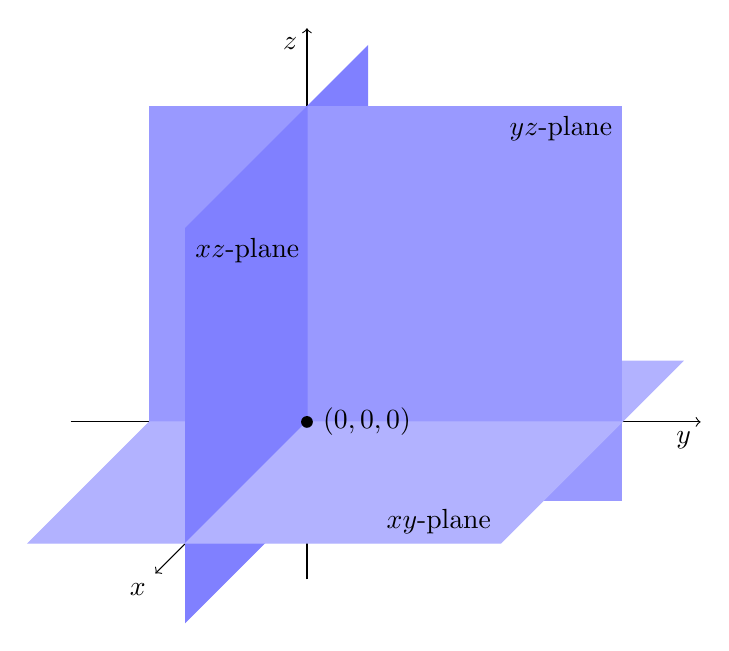
\begin{tikzpicture}
	\draw[->](-3,0,0)--(5,0,0) node[below left]{$y$};
    \draw[->](0,-2,0)--(0,5,0) node[below left]{$z$};
    \draw[->](0,0,-2)--(0,0,5) node[below left]{$x$};
       
    \filldraw[blue!30!white] (0,0,0)--(0,0,-2)--(4,0,-2)--(4,0,0)--cycle;
   \filldraw[blue!50!white] (0,-1,-2)--(0, 4, -2)--(0,4,0)--(0,-1,0)--cycle;
    \filldraw[blue!40!white] (-2,4,0)--(4,4,0)node[black, below left]{$yz$-plane}--(4,-1,0)--(-2,-1,0)--cycle;
    \filldraw[blue!30!white] (0,0,0)--(0,0,4)--(-2,0,4)--(-2,0,0)--cycle;
    \filldraw[blue!50!white] (0,-1,0)--(0, 4, 0)--(0,4,4)node[black, below right]{$xz$-plane}--(0,-1,4)--cycle;
    \filldraw[blue!30!white] (0,0,0)--(0,0,4)--(4,0,4)node[black, above left]{$xy$-plane}--(4,0,0)--cycle;
     
     \node[fill,circle,inner sep=1.5pt,label={right:$(0,0,0)$}] at (0,0,0) {};
\end{tikzpicture}
\end{image}



The set of all ordered $n$-tuples $(x_1, x_2, \ldots, x_n)$, where $x_i$ is a real number for $1\leq i\leq n$ is called $\RR^n$.
$$\RR^n=\{(x_1, x_2,\ldots,x_n)|x_i\in \RR\, \text{for}\, 1\leq i\leq n\}$$
The point $(0,0,\ldots, 0)$ in $\RR^n$ is called the {\it origin}. 

$\RR^n$ cannot be visualized for $n>3$, but many familiar ideas, such as the distance formula, can be generalized to $\RR^n$. 
 

\section*{Practice Problems}
\begin{problem}
Find the coordinates of each point.

  \begin{image}[4.5in]
\begin{tikzpicture}[x=0.5cm,y=0.5cm,z=0.3cm]
% The axes
\draw[->] (xyz cs:x=-13.5) -- (xyz cs:x=13.5) node[above] {$y$};
\draw[->] (xyz cs:y=-13.5) -- (xyz cs:y=13.5) node[right] {$z$};
\draw[->] (xyz cs:z=13.5)--(xyz cs:z=-13.5) node[below] {$x$} ;
% The thin ticks
\foreach \coo in {-13,-12,...,13}
{
  \draw (\coo,-1.5pt) -- (\coo,1.5pt);
  \draw (-1.5pt,\coo) -- (1.5pt,\coo);
  \draw (xyz cs:y=-0.15pt,z=\coo) -- (xyz cs:y=0.15pt,z=\coo);
}

% Dashed lines for the points P
\draw[dashed,red] 
  (xyz cs:z=-5) -- 
  +(0,10) coordinate (u) -- 
  (xyz cs:y=10) -- 
  +(5,0) -- 
  ++(xyz cs:x=5,z=-5) coordinate (v) --
  +(0,-10) coordinate (w) --
  cycle;
\draw[dashed,red] (u) -- (v);
\draw[dashed,red] (5,10) -- (5,0) -- (w);

% Dots and labels for P
\node[fill,circle,inner sep=1.5pt,label={right:$P$}] at (v) {};

% Dashed lines for the points Q
\draw[dashed,blue] 
  (xyz cs:z=6) -- 
  +(0,2) coordinate (u1) -- 
  (xyz cs:y=2) -- 
  +(3,0) -- 
  ++(xyz cs:x=3,z=6) coordinate (v1) --
  +(0,-2) coordinate (w1) --
  cycle;
\draw[dashed,blue] (u1) -- (v1);
\draw[dashed,blue] (3,2) -- (3,0) -- (w1);

% Dots and labels for Q
\node[fill,circle,inner sep=1.5pt,label={right:$Q$}] at (v1) {};

% Dashed lines for the points R
\draw[dashed] 
  (xyz cs:z=-3) -- 
  +(0,-8) coordinate (u2) -- 
  (xyz cs:y=-8) -- 
  +(-5,0) -- 
  ++(xyz cs:x=-5,z=-3) coordinate (v2) --
  +(0,8) coordinate (w2) --
  cycle;
\draw[dashed] (u2) -- (v2);
\draw[dashed] (-5,-8) -- (-5,0) -- (w2);

% Dots and labels for R
\node[fill,circle,inner sep=1.5pt,label={left:$R$}] at (v2) {};

\end{tikzpicture}
\end{image}
Answer:
  $$P(\answer{5}, \answer{5}, \answer{10})$$
 
  $$Q(\answer{-6}, \answer{3}, \answer{2})$$

  $$R(\answer{3}, \answer{-5}, \answer{-8})$$

\end{problem}

\begin{problem}
Imagine that a midday sun is shining directly down on the line segment connecting the origin with the point $(3,4,7)$. What is the length of the shadow (projection) that is formed in the $(x,y)$ plane?

Answer: The length of the shadow is
$$\answer{5}$$
\end{problem}





\end{document} 
